%%&xelatex
\documentclass[PHD]{sysuthesis}
\usepackage[noindent]{ctex}
\usepackage{xeCJK}
\usepackage{setspace}
%\usepackage[BoldFont]{xeCJK}  windows下可以选择使用这个package
%\usepackage{layout}
\usepackage{indentfirst}% not needed if xecjk
\usepackage{ifthen}
\usepackage{dcolumn}	% 
\usepackage{multirow}	%
\usepackage{mdwlist}	% 
\usepackage{verbatim}	% 
\usepackage{bm}
\usepackage{diagbox}
\usepackage{url}
\usepackage{float}
\usepackage{amsmath}
\usepackage{amsthm}
\DeclareMathOperator{\diff}{d\!}
\DeclareMathOperator{\ee}{e}
\DeclareMathOperator{\imag}{i}
\usepackage{amsfonts}
\usepackage{amssymb}	% conflict with xunicode, thus go before it
\usepackage{xltxtra}
\usepackage{rotating}
\usepackage{xunicode}
\usepackage[justification=centering]{caption}
\usepackage[oldenum]{paralist}
\usepackage{enumerate}
\usepackage{url}
\usepackage{algorithmic}
\usepackage[shortlabels]{enumitem}
\usepackage{subfigure}
\usepackage[ruled,vlined]{algorithm2e}
\usepackage{tikz}
\usepackage{amsbsy}
\usepackage{amsmath}
\usepackage{pgfplots}
\usepackage{subfigure}
\usepackage{booktabs}
\usepackage{fontspec}	%[no-math]
\defaultfontfeatures{Mapping=tex-text}
\newcommand{\captionvspace}{\vspace{1em}}
%\setCJKmainfont{SimSun}  
%\setCJKsansfont{SimHei} 

\setCJKmonofont{STFangsong}

\usepackage{graphicx}
\graphicspath{{other/}}
\usepackage[abs]{overpic}\setlength\unitlength{1bp}
\usepackage{tikz}	% great picture package
\usetikzlibrary{shapes.multipart}
\usetikzlibrary{decorations.pathmorphing}
\usetikzlibrary{decorations.shapes}
\usetikzlibrary{shapes.geometric}
\usetikzlibrary{shapes.symbols}
\usepackage[version=3]{mhchem}	% \ce{} for typesetting chemical molecular
\usepackage{hyperref}	% hyperref to URL or internal target
\hypersetup{
	%unicode,	% not use if XeLaTeX
	%bookmarks,	% used by default
	%CJKbookmarks,	% produce bookmarks localized for CJK, e.g., GB2312
	colorlinks=false,	% for printing with gray printer
	%linkcolor=blue,
	%citecolor=blue,
	%urlcolor=blue,
	plainpages=true,
	pdfauthor={},
	pdftitle={},
	pdfview=FitH,
	pdfpagemode=UseOutlines
}
\usepackage{pdfpages}	% 并入答辩委员们签了名的扉页扫描版 
\newtheorem{theorem}{\heiti{定理}}
\newtheorem{lemma}{\heiti{引理}}
\newtheorem{problem}{\heiti{问题}}
\newtheorem{definition}{\heiti{定义}}
\newtheorem{example}{\heiti{例子}}
\let\proof\relax
\let\endproof\relax
\newenvironment{proof}{{\noindent\heiti 证明:}}{\hfill $\square$\par}
\newcommand{\SL}[1]{\textcolor{red}{\textbf{[Todo: #1]}}}
\newcommand{\tmop}[1]{\ensuremath{\operatorname{#1}}}
%matrix & vector
\newcommand*{\mat}[1]{\bm{\mathbf{#1}}}
%set
\newcommand*{\set}[1]{\mathcal{#1}}
%function or variable
\newcommand*{\fun}[1]{\mathit{#1}}
%constant
\newcommand*{\con}[1]{\mathnormal{#1}}
\DeclareMathOperator{\Tr}{Tr}
\newcommand{\Print}{\boolean{true}}%如果 false, 则会并入扉页扫描版 
\makeatletter
\newcommand{\AAstar}{\@ifstar{AA**}{AA}}	% 定义 \foo 和 \foo* 命令。
\def\@cite#1#2{\textsuperscript{[{#1\if@tempswa , #2\fi}]}}
\makeatother
\newcommand{\Verbatiminput}[1]{\noindent\rule{\textwidth}{2pt}{%
	\small\linespread{0.9}\verbatiminput{#1}
	}\noindent\rule{\textwidth}{2pt}}
\newcommand{\Tips}[1]{\textcolor{red}{\textbf{[Tips: #1]}}}
\renewcommand{\cleardoublepage}\clearpage
%如下命令的格式为{中文}{英文},保证全文统一。
\title{
}{ Image Style Conversion using Cycle-Consistent Adversarial Networks}
\author{X\quad X\quad X}{XXX}
\major{XXX}{}
\minor{}
\school{}
\supervisor{}{}
\date{}


\begin{document}

\pagestyle{empty}%
\ifthenelse{\Print}{\maketitlepage[%
	\begin{flushleft}
		\sysufig
		\begin{tabular}{rl@{}l}
			\hspace{50mm}	&	&\\
			\\
			\\
			\\
			院系:		& \underline{\qquad\qquad 数据科学与计算机学院\qquad\qquad\qquad\qquad}	&\\
			\\ \vspace{4mm}
			专业:		&\underline{\qquad\qquad       通信软件   \qquad\qquad\qquad\qquad\qquad\qquad\qquad}	&	\vspace{3mm}\\
			姓名:		&\underline{\qquad\qquad        周芙蓉     \qquad\qquad\qquad\qquad\qquad\qquad\qquad\quad}	&\\ 
			\\ 
			学号:&\underline{\qquad\qquad             16341023     \qquad\qquad\qquad\qquad\qquad\qquad\qquad}	&\\ 
			\\ 
%			&\underline{\qquad\qquad\qquad\qquad\qquad\qquad\qquad}	&\\ 
		\end{tabular}

	\end{flushleft}]}{\includepdf{main_title.pdf}}% 生成扉页或并入扫描版
%\begin{figure}[!t]
%	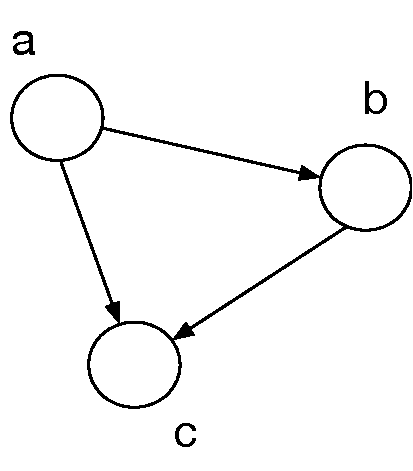
\includegraphics[width=0.25\textwidth]{images/PGM1.pdf}
%\end{figure}
%论文原创性声明和论文版权使用授权书
%\frontmatter
%\ifthenelse{\Print}{{%
\ttfamily\large%
\renewcommand{\baselinestretch}{1.5}%
\setlength{\parindent}{2em}%

\begin{center}
论文原创性声明
\end{center}\vspace{5ex}

本人郑重声明:所呈交的学位论文,是本人在导师的指导下,独立进行研究工作所取得的成果。除文中已经注明引用的内容外,本论文不包含任何其他个人或集体已经发表或撰写过的作品成果。对本文的研究作出重要贡献的个人和集体,均已在文中以明确方式标明。本人完全意识到本声明的法律结果由本人承担。
\vspace{5ex}

\hspace*{\stretch{5}}%
\begin{minipage}{0.6\textwidth}
\begin{tabular}{r@{}l}
学位论文作者签名:	&	\\
日期:			&\hspace{1em}年\hspace{1em}月\hspace{1em}日\\
\end{tabular}
\end{minipage}

\vspace{12em}
\begin{center}
学位论文使用授权声明
\end{center}
\vspace{5ex}

本人完全了解中山大学有关保留、使用学位论文的规定,即:学校有权保留学位论文并向国家主管部门或其指定机构送交论文的电子版和纸质版,有权将学位论文用于非赢利目的的少量复制并允许论文进入学校图书馆、院系资料室被查阅,有权将学位论文的内容编入有关数据库进行检索,可以采用复印、缩印或其他方法保存学位论文。

保密论文保密期满后,适用本声明。
\vspace{6ex}

\noindent%
\begin{minipage}{0.53\textwidth}
\begin{tabular}{r@{}l}
学位论文作者签名:	&	\\
日期:			&\hspace{1em}年\hspace{1em}月\hspace{1em}日\\
\end{tabular}
\end{minipage}\hspace{\stretch{1}}%
\begin{minipage}{0.46\textwidth}
\begin{tabular}{r@{}l}
导师签名:		&	\\
日期:			&\hspace{1em}年\hspace{1em}月\hspace{1em}日\\
\end{tabular}
\end{minipage}
}
}{%
%	\includepdf{main_declare.pdf}}% 生成原创性声明或并入扫描版
%\cleardoublepage\pagestyle{headings}\setcounter{page}{1}\pagenumbering{Roman}%

%中英文摘要



\begin{abstract2}[english]
    Image style conversion refers to the conversion of image content from one domain to another.
    This tasks generally require paired pictures with the same con- tent in the both domains as training data. 
    Such as pix2pix[7], but this pair of training data is difficult to obtain. 
    The innovation of CycleGAN is that can migrate picture content from the source domain 
    to the target domain without paired training data. 
    The Generated Confrontation Network (GAN) consists of two subnetworks: a generator and a recognizer.
    The input to the generator is a random noise or condition vector 
    and the output is the target image. 
    The recognizer is a classifier, the input is an image, 
    and the output is whether the image is a real image. 
    In the training process, the generator and 
    the recognizer enhance their ability through continuous mutual game.

\keywordenglish{Computer Vision , Pattern Recognition, computer science}
\end{abstract2}


%目录,自动生成,不用修改这里的任何东西。
\setcounter{page}{1}\pagenumbering{roman}%
\clearpage\setcounter{tocdepth}{1}%
\tableofcontents
%\clearpage\listoffigures
%\clearpage\listoftables


%正文
\mainmatter
%\layout
\large
%%!TEX root = ./../main.tex
\chapter*{\heiti 主要符号对照表}

\begin{table}[htb]
	\label{notations}
	\begin{tabular}{@{~}ll}
		${G}$ & 普通网络\\
		$\set{G}$ & 属性网络\\
		$\set{G_A}$ & 属性增广网络\\
		$\set{V}$ &  节点的集合\\
		$\set{V_A}$ &  属性增广节点的集合\\
		$\set{A}$ &  属性的集合\\
		$\set{E}$ &  边的集合\\
		$\set{E_A}$ &  节点-属性关联集合\\
		$N=|\set{V}|$ &  节点的数量\\
		$F=|\set{A}|$ &  属性的数量\\
		$\set G_{\set S}$ & 节点集合$\set S$ 在图$\set G$中的导出子图\\
		$\set{V}_{\set G_{\set S}}$ & 子图$\set G_{\set S}$的节点集合\\
		$\set{E}_{\set G_{\set S}}$ & 子图$\set G_{\set S}$的边集合\\
		$\set{A}_{\set G_{\set S}}$ & 子图$\set G_{\set S}$的属性集合\\
		$\set{A}_{\set G_{\set S}}(u)$ &  节点$u$在子图$\set G_{\set S}$的属性集合\\
		$\set{N}_{\set G_{\set S}}(u)$ & 节点$u$在子图$\set G_{\set S}$中的邻居集合\\
		$d_{\set G_{\set S}}(u)$ & 节点$u\in \set{V}$在子图${\set G_{\set S}}$中的度\\
		$\Delta$ & 网络中的最大度数\\
		$D$ &  潜在变量的维度\\
		$\mat{A}\in \mathbb{R}^{N \times N}$ &  节点的边权值矩阵\\
		$\mat{X}\in \mathbb{R}^{N \times F}$ &  节点的属性矩阵 \\
		$\set{A}(u)$ & 与节点$u$关联的所有属性集合\\
		$\set{N}(u)$ & 节点$u$的邻居集合\\
		$|\mat{X}|$ & 表示为$\mat{X}$中全体非零元素的数量\\
		$\left\Vert \cdot\right\Vert _{1}$ & 向量的$l1$-范式\\
		$\left\Vert \cdot\right\Vert _\con{F}$ & 矩阵的Frobenius范式\\
	\end{tabular}
\end{table}




\chapter{\heiti \label{ch1}绪论}
\section{\heiti 选题背景与意义}

Handling another style of scene with different styles 
is a time-consuming and laborious task and requires 
a lot of professional drawing skills. 
In order to obtain a high quality picture, 
the original author must carefully draw each line 
and paint each color area of the target scene. 
It appears that existing art editing software and 
algorithms with standard features do not produce 
satisfactory comic effects. Therefore, 
if professional technology can automatically convert 
one style of photo into another, 
it is very helpful for the artist: 
it can save them a lot of time and 
let them focus on More meaningful and creative work
The goal of picture migration is to use 
a paired picture training data set to learn 
the mapping between the input picture 
and the output picture, such as pix2pix\cite{pix2pix}, 
however, there are no paired training data sets for many items.
The innovation of CycleGAN\cite{Cyclegan} is that can migrate 
picture content from the source domain to the target domain 
without paired training data.

\begin{enumerate}[(1)] 
	\item When CycleGAN\cite{Cyclegan} is training, it only needs to 
	input the image of the source domain and the image of the target domain.
	This does not require the source domain to match the image content of the target domain.
	
	\item Based on cyclegan's CariGAN\cite{cGAN}, 
	you can automatically convert live-action photos 
	into formally exaggerated comics without paired images.
	
	\item With CycleGAN, not only convert between two types of images, 
	but also convert between two objects, 
	such as translating one person into another.
	
	
\end{enumerate}


\section{\heiti 国内外研究现状和相关工作}
随着国内外研究者们对图像迁移越来越关注,
出现了一系列的Cyclegan算法。
在这一小节,我们简短的介绍四条相关工作 
(Generative Adversarial Networks (GANs)、
Image-to-Image Translation、
Unpaired Image-to-Image Translation、
Cycle Consistency)
和其国内外研究现状。
\subsection{\heiti Generative Adversarial Networks (GANs)}
Generative Adversarial Networks (GANs)\cite{GAN,GAN1}
have achieved impressive results in image generation\cite{imagegen,imagegen1},
image editing \cite{imgaeedi}, 
and representation learning\cite{imagegen1,replearn}.
The key to the success of GAN is 
the concept of confrontational loss, 
which forces the generated image to be 
indistinguishable from the real image in principle.

\subsection{\heiti Image-to-Image Translation}
The idea of image to image conversion 
is to use a non-parametric texture model\cite{texmodel}
 on a single input-output training image pair. 
 The latest method uses the data set of 
 input and output checks to learn the 
 parameter conversion function through CNN\cite{CNN}. 
 Our approach is based on the "pix2pix"\cite{pix2pix} 
 framework of Isola et al\cite{Isola}.
 It uses conditional generation of the network 
 to learn the mapping from input to output images.


\subsection{\heiti Unpaired Image-to-Image Translation}
The similarity function between the predefined inputs 
and outputs that does not depend on any particular task, 
nor does it assume that we assume that the inputs 
and outputs must be in the same low-dimensional 
embedded space. This makes our approach a 
universal solution for many visual and graphical tasks.

\subsection{\heiti Cycle Consistency}
In target tracking, language translation, 
3D shape registration and so on. 
There are also applications in CNN. 
A similar loss was introduced to push G and F 
to agree with each other.

\section{\heiti 国内外研究现状}
\begin{enumerate}[(1)] 
	\item In 2018, researchers from Tsinghua University,
	 City University of Hong Kong and Microsoft recently 
	 proposed CariGAN\cite{cGAN}, which can automatically 
	 convert live-action photos into formally 
	 exaggerated cartoons without paired images.
	
	\item 
	
	
\end{enumerate}



% \newpage
   %前言,绪论等
\chapter{\heiti \label{ch2}技术背景知识}
\section{\heiti model}

\begin{figure}[thb]
  \centering
    \subfigure{
      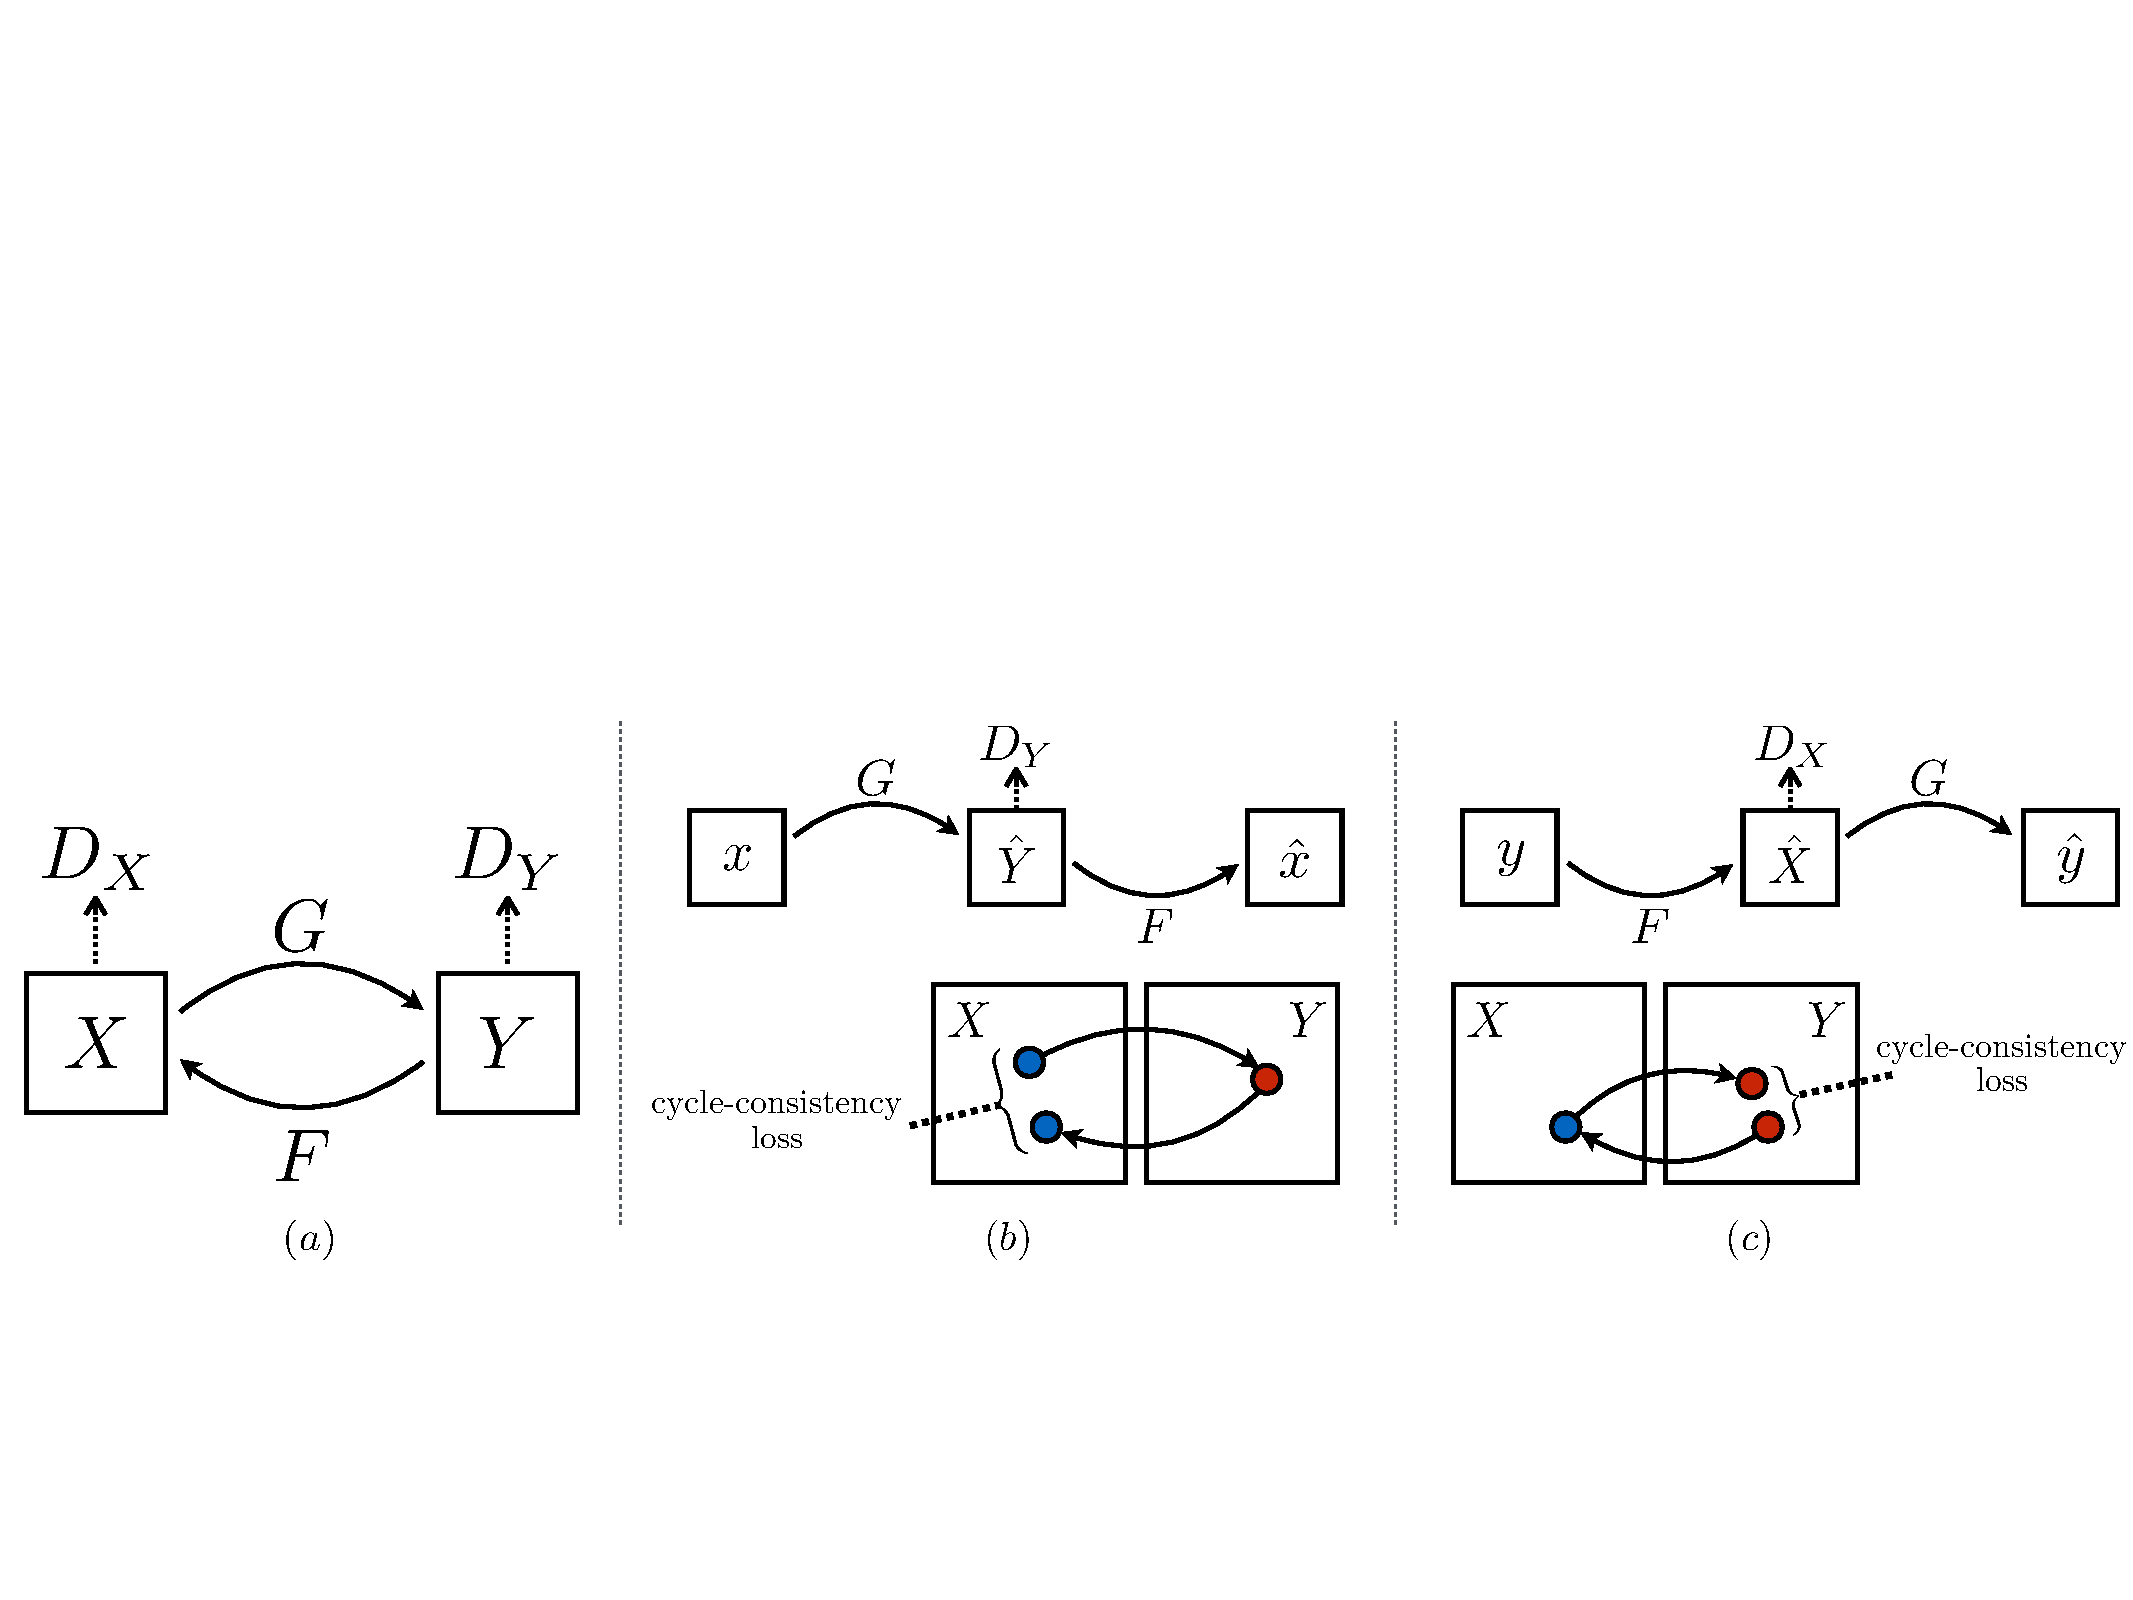
\includegraphics[width=0.9\textwidth]{images/system_diagram_v2.pdf}}
  \caption{CycleGAN is actually an A→B one-way GAN plus a B→A one-way GAN. The two GANs share two generators, each with a discriminator, so adding up to a total of two discriminators and two generators. A one-way GAN has two losses, and CycleGAN adds up to a total of four losses.}
  \label{fig:PGM1}
  \end{figure}

\subsection{\heiti 表示}
Adversarial Loss:For the mapping function G : X → Y and its dis- criminator DY , we express the objective as

\begin{align}
\mathcal{L}_{\text{GAN}}(G,D_Y,X,Y) =  \ \mathbb{E}_{y \sim p_{\text{data}}(y)}[\log D_Y(y)] \nonumber \\
+  \ \mathbb{E}_{x \sim p_{\text{data}}(x)}[\log (1-D_Y(G(x))]
\end{align}

\begin{align}
  \mathcal{L}_{\text{GAN}}(G,D_X,X,Y) =  \ \mathbb{E}_{x \sim p_{\text{data}}(y)}[\log D_X(y)] \nonumber \\
  +  \ \mathbb{E}_{y \sim p_{\text{data}}(x)}[\log (1-D_X(G(x))]
  \end{align}

  Cycle Consistency Loss. The so-called Cycle consistency is to ensure
  
  Forward consistent: x->G(x)->F(G(x))≈x
  
  Backward agreement: y->F(y)->G(F(y))≈y

  We incentivize this behavior using a cycle consistency loss:
 \begin{align}
   \mathcal{L}_{\text{cyc}}(G, F) =  mathbb{E}_{x\sim p_{\text{data}}(x)} [[{F(G(x))-x}]_1] \nonumber \\ 
   + \ \mathbb{E}_{y\sim p_{\text{data}}(y)}[[{G(F(y))-y}]_1]
 \end{align}

 full objective loss function is:
 \begin{align}
  \mathcal{L}(G,F,D_X,D_Y) = \mathcal{L}_{\text{GAN}}(G,D_Y,X,Y) \nonumber \\
  +\ \mathcal{L}_{\text{GAN}}(F,D_X,Y,X) \nonumber \\
  +\  \lambda \mathcal{L}_{\text{cyc}}(G, F)
 \end{align}




\section{\heiti 深度生成模型}
The network architecture of CycleGAN is shown in the figure\ref{fig:1}:

  \begin{figure}
  \centering
\subfigure[]{
  \begin{minipage}[b]{0.9\textwidth}
  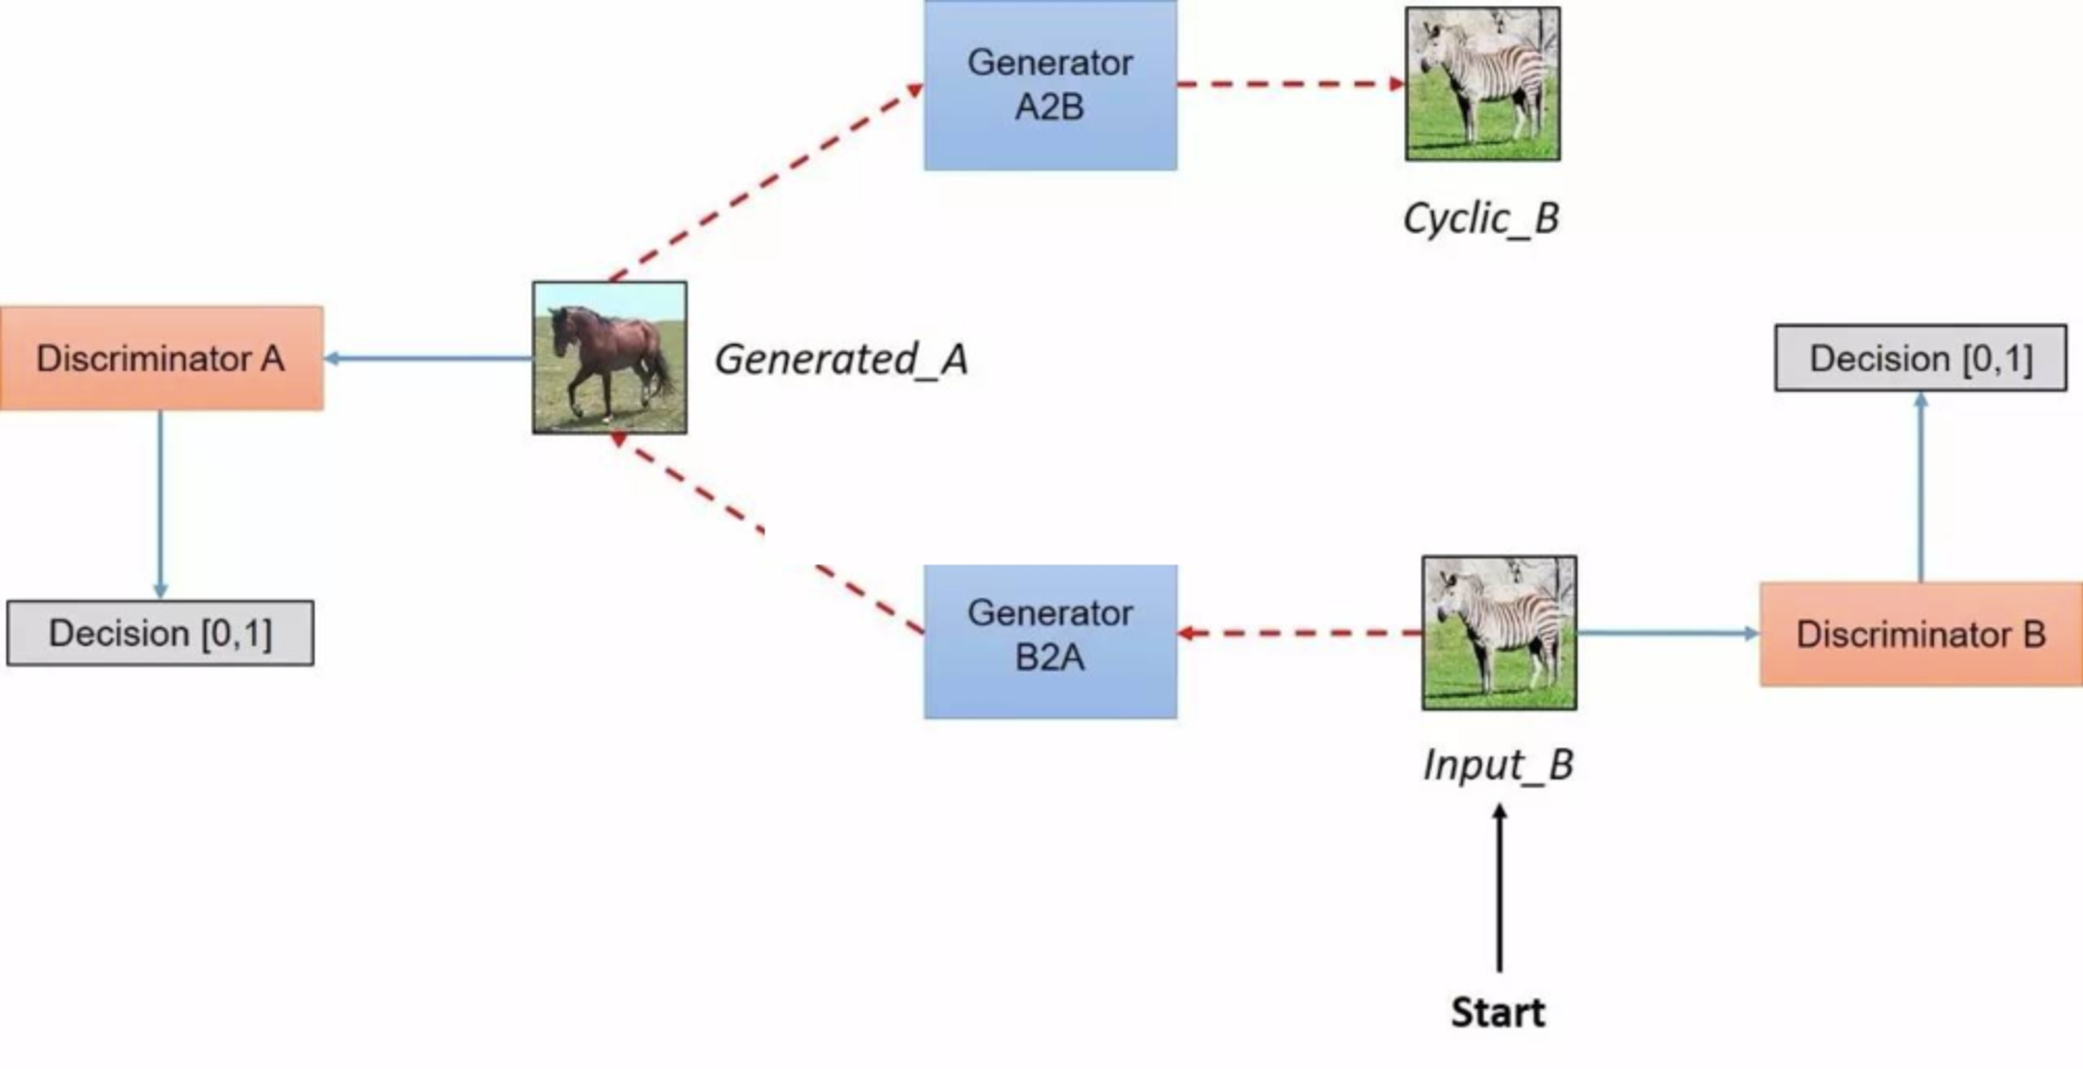
\includegraphics[width=1\textwidth]{images/agr.pdf}
\end{minipage}}
\subfigure[]{
  \begin{minipage}[b]{0.9\textwidth}
  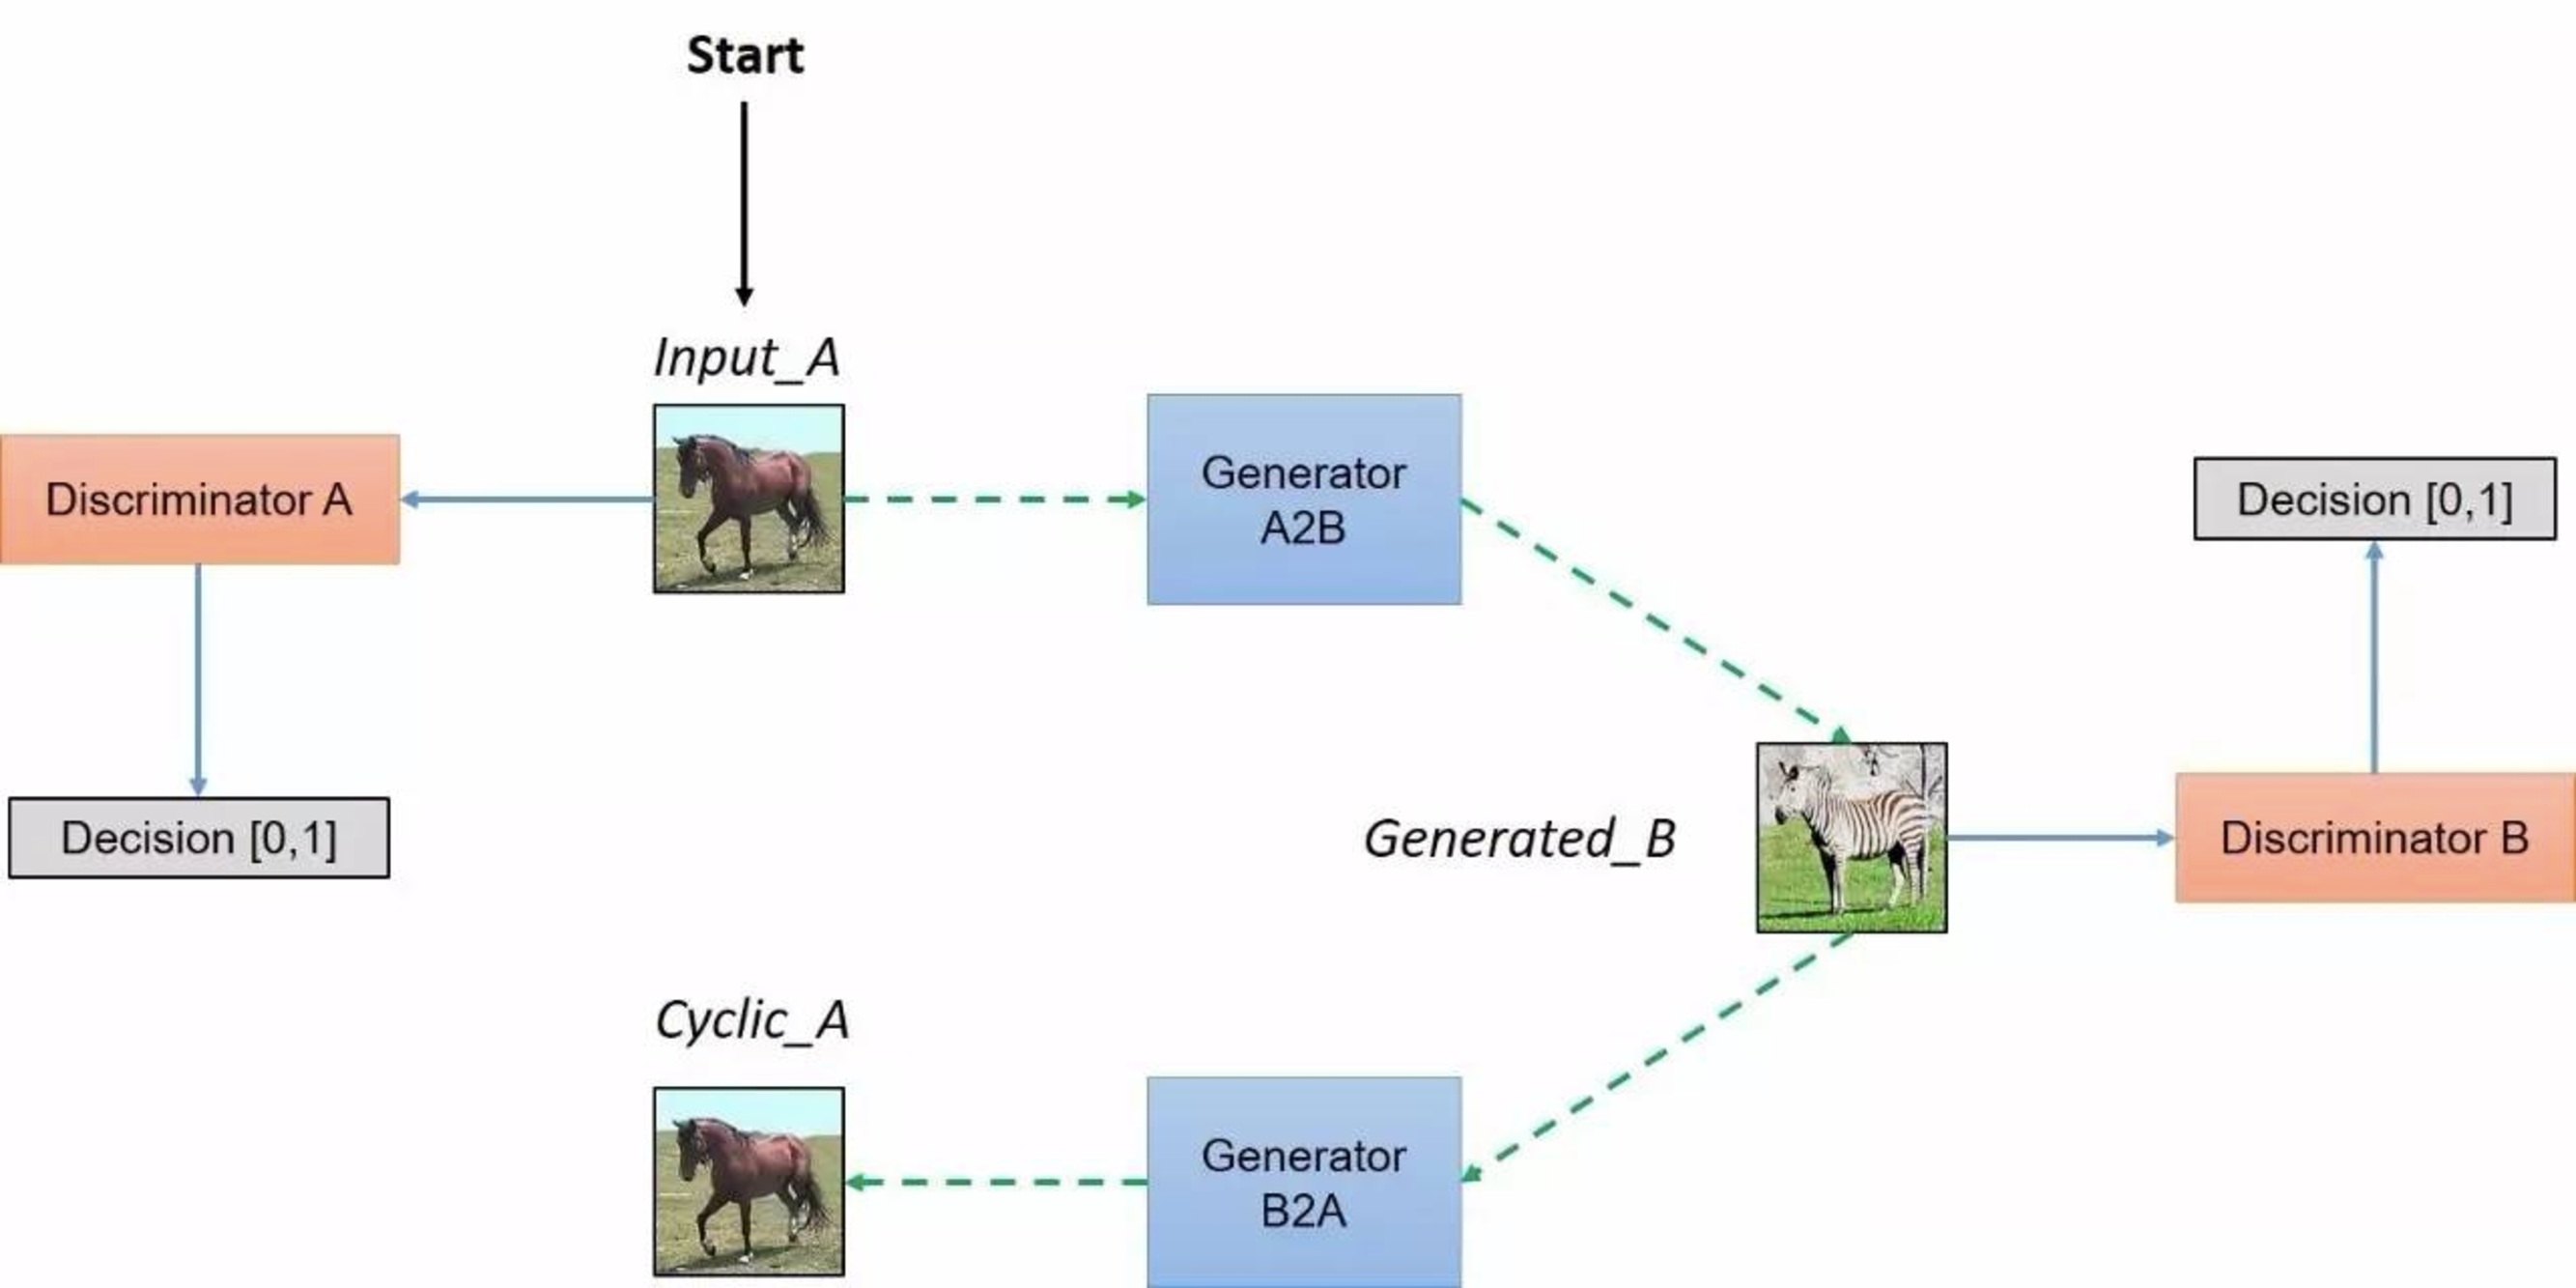
\includegraphics[width=1\textwidth]{images/agr1.pdf}
\end{minipage}} 
\caption{The model acquires an input image from the domain DA, 
which is passed to the first generator GeneratorA→B, 
whose task is to convert a given image from the 
domain DA to an image in the target domain DB. 
This newly generated image is then passed to another generator, 
GeneratorB→A, whose task is to convert back to 
the image CyclicA in the original domain DA,
which can be compared to the autoencoder. 
This output image must be similar to the 
original input image and is used to define 
meaningful mappings that did not exist in the unpaired data set.} 
\label{fig:1}
\end{figure}

    
\chapter{\heiti \label{ch3} 非配对图片的图像迁移算法}

\section{\heiti \label{sec:2.1}算法流程}
\begin{algorithm}[thb]
	\caption{k, is a hyperparameter.We used k = 1, the least expensive option, in our experiments}
    \label{alg}
	\begin{algorithmic}[1]
	\REQUIRE  图片A数据集 $\mathbf{R}$,  图片B数据集 $\mathbf{X}$,迭代次数 n 
    \FOR{$i = 1$ to $n$}
      \STATE\FOR{$i = 1$ to $k$}
      \STATE Sample minibatch of m noise Samples from noise prior Pg(z)
      \STATE Sample minibatch of n examples from data generationg districution Pdata(x)
      \STATE Update the discriminator by ascending its stochastic gradient:
      \STATE \begin{align}
        \bigtriangledown_{\theta_{d}} 1/M \sum_{n=1}^M [\log D(x^{i}) + \log (1-D(G(z^{i})))]
      \end{align}
      \STATE\ENDFOR
      \STATE Sample minibatch of m noise Samples from noise prior Pg(z)
      \STATE Update the discriminator by decending its stochastic gradient:
      \STATE \begin{align}
        \bigtriangledown_{\theta_{g}} 1/M \sum_{n=1}^M \log (1-D(G(z^{i})))
      \end{align}
    \ENDFOR

	\end{algorithmic}
\end{algorithm}

\section{\heiti \label{sec:2.2}实验数据集}

\subsection{\heiti 数据集来源}
本次实验数据集来源为原作者提供的数据集,数据集来源:\url{https://people.eecs.berkeley.edu/~taesung_park/CycleGAN/datasets/}

\section{\heiti \label{sec:2.2}实验结果}
The experimental results are shown in the figure\ref{fig:change}\ref{fig:change2}\ref{fig:loss_200_20}.

\begin{figure}[thb]
\centering
\subfigure{
  \label{subfig:contour-Lastfm-VDCMF-PAKDD}
  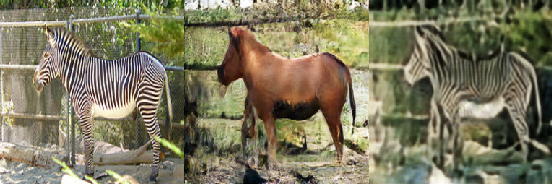
\includegraphics[width=0.65\textwidth]{images/Test_result_86.png}}
  \space \space \space \space \space \space \space
 \subfigure{
  \label{subfig:contour-Epinions-VDCMF-PAKDD}
  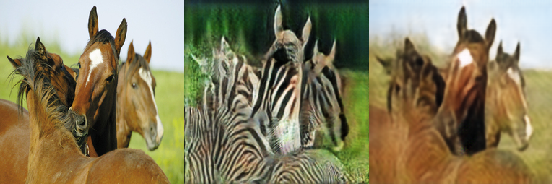
\includegraphics[width=0.67\textwidth]{images/Test_result_2.png}}
\caption{}
\label{fig:change2}
\centering
    \subfigure{
      \label{subfig:contour-Lastfm-VDCMF-PAKDD}
      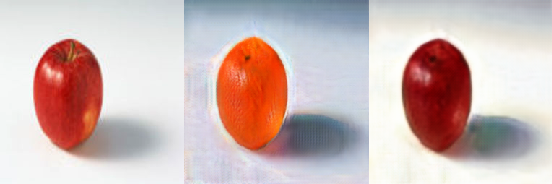
\includegraphics[width=0.65\textwidth]{images/Test_result_164.png}}
      \space \space \space \space \space \space \space
     \subfigure{
      \label{subfig:contour-Epinions-VDCMF-PAKDD}
      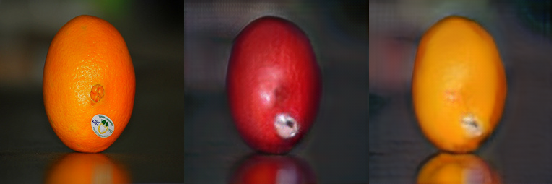
\includegraphics[width=0.67\textwidth]{images/Test_result_235.png}}
  \caption{Basically, the conversion between unpaired images and images has been implemented, but the conversion effect is not very good, and the converted image is not smooth enough. In the pixel processing, our model still needs improvement.}
  \label{fig:change}

      \includegraphics[width=0.67\textwidth]{images/loss200_02.pdf}
  \caption{As the epoch continues to increase,
  the accuracy of GA and GB 
  keep rising and gradually stabilizes.
  the stable values of $D_A$ is about 0.83,
  the stable values of $D_B$ is about 0.76.}
  \label{fig:loss200_02}
\end{figure}



\section{\heiti 不同图像迁移算法性能比较}

As shown in the table\ref{table:performance}, 
Cyclegan basically realizes the conversion 
between unpaired pictures, 
but the image conversion effect is slightly 
worse than other image migration algorithms. 
The results obtained from the experiment do 
not affect the intuitive judgment of the human eye.

\begin{table}[htb]
  \center
  \caption{}
  \label{table:performance}
  \resizebox{1\textwidth}{!}{
  \begin{tabular}{|c|c|c|c|c|c|c|c|c|}
  \hline
   &\multicolumn{1}{|c|}{Map to Photo}& \multicolumn{1}{|c|}{Photo to  Map}\\
  \hline
   & Error rate  &  Error rate\\
  \hline
  CoGAN\cite{CoGAN} & 1.1\% & 1.4\% \\
  SimGAN\cite{SimGAN} &1.6\% & 2.8\% \\
  CycleGAN(our) & 23.6\% &22.4\% \\
  
  \hline
  \end{tabular}
  }
  \end{table}


\section{\heiti 算法参数的影响}
When obtaining the optimal parameters of the model,
 we use the small epoch to continuously test the optimal parameters of the approximation model. 
 Finally, the learning rate is best around 0.002.

\begin{figure}[htbt]
  \centering
    \subfigure{
      \label{subfig:loss200_02}
      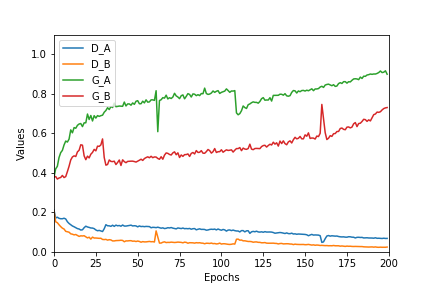
\includegraphics[width=6cm,height = 5cm]{images/loss_200_02.png}}
      \space \space \space \space \space \space \space
     \subfigure{
      \label{subfig:loss20_02}
      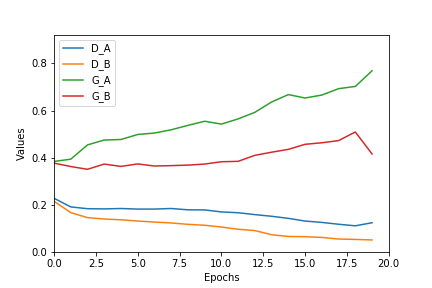
\includegraphics[width=6cm ,height=5cm]{images/loss_20_02.png}}
  \caption{The epoch value increases and 
  the value increases when the 
  accuracy reaches stability.}
  \label{fig:loss_200_20}
  
  \centering
    
     \subfigure{
      \label{subfig:loss20_015}
      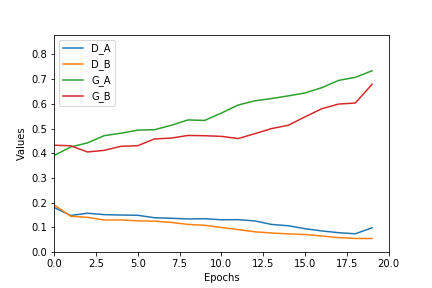
\includegraphics[width=0.67\textwidth]{images/loss_20_015.png}}
      \subfigure{
      \label{subfig:loss20_030}
      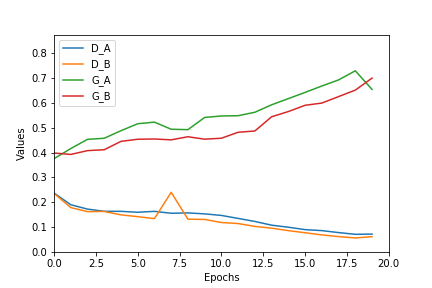
\includegraphics[width=0.67\textwidth]{images/loss_20_030.png}}
  \caption{When the learning rate is equal to 0.003, there is an over-fitting phenomenon. When the learning rate is 0.0015, the image is slightly worse than the learning rate of 0.002.}
  \label{fig:loss_02_015_030}
  
\end{figure}









%\input{mainbody/chapters/chapter3}
\chapter{\heiti \label{ch5}总结}

\section{\heiti \label{sec:5.1}总结}
In this report, we implement the code of 
“Unpaired Image-to-Image Translation 
using Cycle-Consistent Adversarial Networks”. 
The success of our cyclegan model is 
due to the standing of the work of our predecessors.
This recurring experiment gives us a deeper 
understanding of GAN and encourages us to focus on our deep learning.


Code implementation is a fine-tuning, referring \href{https://github.com/eriklindernoren/PyTorch-GAN}{PyTorch-GAN}
and 
\href{https://github.com/junyanz/pytorch-CycleGAN-and-pix2pix}{pytorch-CycleGAN-and-pix2pix}





Since some code lines are too long, the cvpr template cannot display the code properly. The code item address is given below.	\url{https://github.com/zfr0411/CycleGAN} % if need

%引用论文
%\bibliographystyle{unsrt}
\bibliographystyle{sysuthesis}
\bibliography{references}

%附录
%\appendix
%
\chapter{附录}

\section{附录是什么}
\Verbatiminput{}
附录是正文主体的补充。
下列内容可以作为附录:
\begin{enumerate}
\item 攻读学位期间发表的(含已录用,并有录用通知书的)与学位论文相关的
	学术论文目录
\item 由于篇幅过大,或取材于复制件不便编入正文的材料、数据
\item 对本专业同行有参考价值,但一般读者不必阅读的材料
\item 论文中使用的符号意义、单位缩写、程序全文及有关说明书
\item 附件:计算机程序清单、软磁盘、鉴定证书、获奖奖状或专利证书的复印件等
\end{enumerate}


%附加材料
\backmatter


\end{document}
